\documentclass[a4paper, 11pt]{article}
\usepackage[utf8]{inputenc}
\usepackage[left=18mm, right=18mm, top=22mm, bottom=22mm]{geometry}

\usepackage{amsmath,amsfonts,amssymb,bm}
\usepackage[english]{babel}
\usepackage{hyperref}
\usepackage{xcolor}
\usepackage{fancyhdr}
\usepackage{graphicx}
\usepackage{booktabs}
\usepackage{float}
\usepackage{multirow}
\usepackage{caption}
\usepackage{verbatim}  % provides \begin{comment}...\end{comment}

% Preferred style -------------------------------------------------------------
\definecolor{harvardcrimson}{HTML}{8C1D40}
\definecolor{softgrey}{HTML}{F3F3F3}
\definecolor{kwcol}{HTML}{1F4E79}
\definecolor{datablockcol}{HTML}{4B644A}

\hypersetup{
  colorlinks=true,
  linkcolor=harvardcrimson,
  citecolor=harvardcrimson,
  urlcolor=harvardcrimson,
  hypertexnames=false,
}

\pagestyle{fancy}
\fancyhf{}
\rhead{\textcolor{harvardcrimson}{\textbf{Buzzard mock cluster data vector}}}
\lhead{\textcolor{harvardcrimson}{\textbf{X.\,Tang}}}
\cfoot{\thepage}
\renewcommand{\headrulewidth}{0.4pt}
\renewcommand{\footrulewidth}{0.4pt}
\setlength{\headheight}{14pt}
\renewcommand{\baselinestretch}{1.12}

% algorithm2e ----------------------------------------------------------------
\usepackage[ruled,vlined,linesnumbered]{algorithm2e}
\SetKwInput{KwData}{Inputs}
\SetKwInput{KwResult}{Outputs}
\SetKwInput{KwConfig}{Knobs}
\SetKwFor{PerZ}{for each}{do}{end}
\SetKwProg{Fn}{Function}{:}{}
\DontPrintSemicolon

% Custom commands ------------------------------------------------------------
\newcommand{\lob}{\lambda^{\rm ob}}
\newcommand{\ltr}{\lambda^{\rm tr}}
\newcommand{\lrm}{\lambda^{\rm RM}}
\newcommand{\zob}{z^{\rm ob}}
\newcommand{\ztr}{z^{\rm tr}}
\newcommand{\zrm}{z^{\rm RM}}
\newcommand{\hMpc}{h^{-1}\,\mathrm{Mpc}}
\newcommand{\hMsun}{h^{-1}\,M_{\odot}}
\newcommand{\Bsel}{\mathcal{B}_{\rm sel}}
\newcommand{\Bcal}{\mathcal{B}}
\newcommand{\modname}[1]{\textcolor{kwcol}{\texttt{#1}}}
\newcommand{\blk}[1]{\textcolor{datablockcol}{\texttt{#1}}}
\newcommand{\pyfile}[1]{{\small\texttt{#1}}}

\title{\vspace{-4ex}\huge \textbf{Buzzard cluster mock data vector with}\\[0.5ex]
       \Large \textbf{optical-selection effects: forward model,
                      analytical and empirical $\Bsel$ closures}}
\author{X.\,Tang}
\date{2026-05-28}

\begin{document}
\maketitle

\begin{abstract}
This document is the technical reference for
\modname{MockDataVector.ipynb}: a Buzzard-halo DES~Y3-like cluster
mock that layers the Costanzi+2026 (C26) optical selection systematics on
top of the raw simulation outputs, on the DES~Y1 cluster binning
($\lambda \in \{20, 30, 45, 60, \infty\}$, $z \in \{[0.20, 0.33),\,
[0.37, 0.50),\, [0.50, 0.65)\}$ — the standard DES~Y1 redshift edges
with the upper edge of $z_0$ pulled in from $0.35 \to 0.33$ and the
lower edge of $z_1$ pushed out from $0.35 \to 0.37$ to skip the
Buzzard $0.33 \le z < 0.37$ box-junction seam). The data vector is constructed along
\emph{two parallel routes} that share the same Costanzi+2019 (C19) forward model upstream
and the same lensing geometry: an \textbf{analytical} closure based on the
C26 Appendix~C Eq.~C1 fitting function applied to the C19-binned stack
(cheap enough for an MCMC chain), and an \textbf{empirical} ratio that
stacks on the catalog redMaPPer outputs $(\texttt{LAMBDA\_CHISQ},
\texttt{Z\_LAMBDA})$ and divides by a $(\log M, \ztr)$-matched random
reference (Wu+2022, Costanzi+2026). The notebook also produces a binned
number-count vector $N(\lob, \zob)$. Member-galaxy contamination
(boost factor) is injected from the published DES~Y1 measurements
(McClintock+2019), so the saved final shear
$\gamma_t^{\rm mock,obs} = \Delta\Sigma_{\rm obs,C1}/B_{\rm Y1}\cdot\Sigma_{\rm crit}^{-1}$
mimics the raw uncorrected DES~Y1 data vector. All outputs are saved to
\pyfile{output/MockDataVector.npz}; the headline plots embedded in
this document live in \pyfile{output/figs/}.
\end{abstract}

\tableofcontents
\vspace{1em}

% ============================================================================
\section{Pipeline topology}
\label{sec:topology}

The notebook executes the following stages in order:

\begin{center}
\fbox{\parbox{0.95\linewidth}{\centering
\modname{halo\_load} $\to$ \modname{photoz\_proxy} $\to$
\modname{sample\_lambda\_true} $\to$ \modname{sample\_lambda\_obs} $\to$
\modname{lensing\_inputs} $\to$ \modname{number\_counts} $\to$
\modname{analytical\_C1} $\to$ \modname{empirical\_mass\_match} $\to$
\modname{save\_npz}}}
\end{center}

The first four stages are the C19 forward model: select host halos above
$\log_{10} M_{\rm vir} = 13$ in $z \in [0.20, 0.65]$ (with the Buzzard
$0.33 \le z < 0.37$ box seam excised), add a DES~Y3-like Gaussian photo-$z$
scatter to produce $\zob$, and draw $\ltr$ and $\lob$ from the C26/C19
kernels. \modname{lensing\_inputs} centralises the per-halo profiles and
$\Sigma_{\rm crit}^{-1}$ table, plus the catalog redMaPPer columns
($\texttt{LAMBDA\_CHISQ}, \texttt{Z\_LAMBDA}$) used by the empirical route.
The two lensing-data-vector stages are independent and produce their
outputs on the same DES~Y1 binning so the user can compare them
side-by-side. The final stage persists everything to
\pyfile{output/MockDataVector.npz}.

% ============================================================================
\section{Shared conventions}
\label{sec:conventions}

\paragraph{Cosmology.} \texttt{FlatLambdaCDM(H0=70, Om0=0.3, Ob0=0.046,
Tcmb0=2.725)} via \texttt{astropy.cosmology}, matching the Buzzard
simulation cosmology used by the upstream halo catalogue.

\paragraph{Units.} Per-halo $\Sigma, \Delta\Sigma$ are stored in physical
$M_\odot/\mathrm{pc}^2$; radii \blk{rp\_phys\_mpc} (from
\pyfile{src/radial\_bins\_phys\_mpc.py}) are in physical Mpc, with $N_R = 15$
log-spaced bins between $0.0323$ and $30\,\mathrm{Mpc}$. Halo masses
\blk{Mvir} are in $\hMsun$.

\paragraph{Halo selection.} Mirrors \pyfile{0-MakeMock.ipynb}:
\texttt{pid == -1} (host halos only), $0 \le \cos i \le 1$ (measured), drop
the $0.33 \le z < 0.37$ simulation-box seam, then require $0.20 \le \ztr
\le 0.65$ and $\log_{10} M_{\rm vir} \ge 13$. Yields $\sim 5.83 \times
10^5$ halos.

\paragraph{DES~Y1 binning (used everywhere).} Both abundance and lensing
bins follow the DES~Y1 cluster edges (Costanzi+2019, McClintock+2019),
with the central two redshift edges shifted inward by $\pm 0.02$ to
skip the Buzzard box-junction seam at $0.33 \le z < 0.37$:
\begin{equation*}
  \texttt{LBDBINS}    = \{20,\, 30,\, 45,\, 60,\, 500\},\qquad
  \texttt{ZMIN\_LIST} = \{0.20,\, 0.37,\, 0.50\},\qquad
  \texttt{ZMAX\_LIST} = \{0.33,\, 0.50,\, 0.65\}.
\end{equation*}
The $500$ caps the open $[60, \infty)$ richness range. There are
$N_\lambda \times N_z = 4 \times 3 = 12$ bins. The seam volume is
$\sim 5\%$ of $z_0$ and $\sim 13\%$ of $z_1$ on the published Y1
edges; pulling the bin edges inward eliminates the bias on $N(\lob,
\zob)$ at the cost of a small mismatch with the Y1-published bin
ranges (negligible on $B_\mathrm{sel}$, $B_\mathrm{data}$, and the
shear data vector since these are intensive quantities).

\paragraph{Photo-$z$ proxy.} Per-halo Gaussian
\begin{equation}
  \zob = \ztr + \sigma_z(1 + \ztr)\,\mathcal N(0, 1),\quad \sigma_z = 0.01,
  \label{eq:photoz-proxy}
\end{equation}
clipped at $\zob \ge 0.02$. Stand-in for the DES~Y3 redshift kernel of
Myles+2021; captures the dominant scatter but not the tails.

\paragraph{Random seeds.} A single
\texttt{numpy.random.default\_rng(seed=42)} is shared across the forward
model. The MC-vs-PDF sanity histogram uses \texttt{seed=123}; the §8.1
bootstrap uses \texttt{seed=0}.

% ============================================================================
\section{The intrinsic mass--richness relation (C26 Eq.~15)}
\label{sec:mass-richness}

\modname{Path}\,\pyfile{src/costanzi\_selection.py}
(\texttt{l\_sat}, \texttt{l\_tr}, \texttt{sample\_lambda\_true}).

The intrinsic richness $\ltr$ of a halo (the true number of red-sequence
satellite galaxies hosted by the halo, plus the central galaxy) is
modelled as a halo central plus a Poisson satellite count. The mean
satellite count $\bar\lambda_{\rm sat}(M, z)$ follows C26 Eq.~15,
\begin{equation}
\label{eq:lsat}
  \bar\lambda_{\rm sat}(M, z)
  = \left( \frac{M - M_{\rm min}}{M_{\rm pivot}} \right)^{\!\alpha}
        \left( \frac{1+z}{1+z_{\rm piv}} \right)^{\!\epsilon},
\end{equation}
clipped to zero for $M < M_{\rm min}$. The mean intrinsic richness adds
the central galaxy when the halo is above threshold:
\begin{equation}
  \label{eq:ltr-mean}
  \langle\ltr | M, z\rangle =
  \begin{cases}
    1 + \bar\lambda_{\rm sat}(M, z), & M \ge M_{\rm min}, \\
    0,                                & M < M_{\rm min}.
  \end{cases}
\end{equation}

The DES~Y1 NC$+3{\times}2$pt best-fit constants, hard-coded in
\pyfile{src/costanzi\_selection.py}:
\begin{equation*}
  \log_{10} M_{\rm min} = 11.385,\quad
  \alpha = 0.859,\quad
  \log_{10} M_1 = 12.696,\quad
  \sigma_{\rm intr} = 0.181,\quad
  \epsilon = 0.284,\quad
  z_{\rm piv} = 0.4544,
\end{equation*}
with $M_{\rm pivot} = M_1 - M_{\rm min}$.

The per-halo $\ltr$ value is drawn (C26 Sec.~III) by
\textit{(i)} broadening the Poisson rate $\bar\lambda_{\rm sat}$ with a
multiplicative log-normal of width $\sigma_{\rm intr}$,
\textit{(ii)} drawing an integer satellite count, and
\textit{(iii)} adding 1 for the central galaxy if the halo is above
$M_{\rm min}$:
\begin{equation*}
  \tilde\lambda_{\rm sat} = \bar\lambda_{\rm sat}(M, z)\,
    \exp\!\left[\sigma_{\rm intr}\,\mathcal N(0, 1)
    - \tfrac{1}{2}\sigma_{\rm intr}^2\right],\qquad
  N_{\rm sat} \sim \mathrm{Poisson}(\tilde\lambda_{\rm sat}),\qquad
  \ltr = N_{\rm cen}(M) + N_{\rm sat},
\end{equation*}
where $N_{\rm cen}(M) = 1$ if $M \ge M_{\rm min}$ and $0$ otherwise.

% ============================================================================
\section{The projection kernel (C19 Eq.~6)}
\label{sec:projection}

\modname{Path}\,\pyfile{src/costanzi\_selection.py}
(\texttt{projection\_params}, \texttt{sample\_lambda\_obs}). C19 Eq.~6 is a
Gaussian-core $+$ exponentially-modified-Gaussian (EMG) mixture:
\begin{equation}
\label{eq:c19-eq6}
  P(\lob | \ltr, z)
  = (1 - f_{\rm prj})\, \mathcal N(\mu, \sigma)
       + f_{\rm prj}\, \mathrm{EMG}(\mu, \sigma, \tau).
\end{equation}
The four parameters $\{\mu, \sigma, \tau, f_{\rm prj}\}$ depend on
$\ltr$ with $z$-dependent coefficients calibrated from SDSS redMaPPer
(C19 Appendix~A, Eq.~A8):
\begin{equation}
\label{eq:c19-a8}
\begin{aligned}
  \mu(\ltr, z)         &= a_\mu(z) + b_\mu(z)\,\ltr,
  & \sigma(\ltr, z)     &= b_\sigma(z)\,(\ltr)^{a_\sigma(z)}, \\
  \tau(\ltr, z)        &= b_\tau(z)\,(\ltr)^{-a_\tau(z)},
  & f_{\rm prj}(\ltr, z)&= b_{f_{\rm prj}}(z)\,\big(1 + e^{-\ltr}\big)^{-a_{f_{\rm prj}}(z)}.
\end{aligned}
\end{equation}
The 15 rows of \pyfile{data/prj\_params\_DESY3\_lss\_lin\_dep\_getdist\_v1.txt}
are interpreted as posterior samples and collapsed to the posterior mean
via \texttt{load\_prj\_posterior\_mean}.

The mixture is sampled directly using the EMG = $\mathcal N(\mu,\sigma) +
\mathrm{Exp}(1/\tau)$ representation, avoiding a closed-form EMG density
evaluation in the sampling path. The closed form is used only for the
sanity overlay below.

\paragraph{Sanity check 1 --- MC draws vs analytical kernel.}
Histogram repeated \texttt{sample\_lambda\_obs} draws at fixed
$(\ltr, z)$ and overlay the closed-form C19 PDF; they should agree within
Poisson noise.

\begin{figure}[H]
\centering
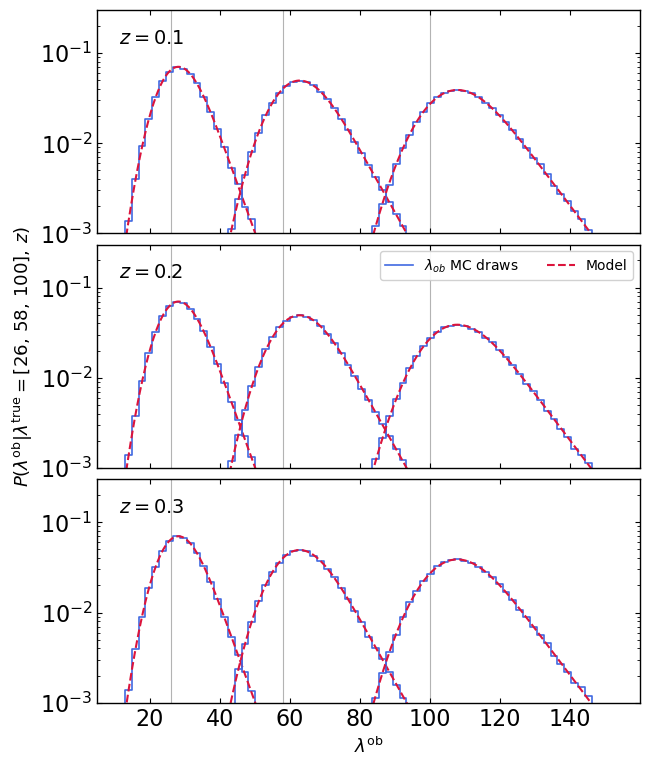
\includegraphics[width=0.55\linewidth]{../output/figs/01_projection_kernel_mc_vs_pdf.png}
\caption{MC draws of $\lob$ from \texttt{sample\_lambda\_obs} (blue
histograms) overlaid with the closed-form PDF of
Eq.~\ref{eq:c19-eq6} (red dashed) at three reference redshifts and
three intrinsic richnesses. The two agree within Poisson noise across
the bulk and the tail.}
\label{fig:mc-vs-pdf}
\end{figure}

\paragraph{Sanity check 2 --- Gaussian core + EMG tail decomposition.}
Same kernel as Eq.~\ref{eq:c19-eq6}, split into the two physical
components. At large $\ltr$
the EMG tail dominates the high-$\lob$ side and drives the projection
bias; this is what the analytical $\Bcal_{\rm sel,C1}$ of \S\ref{sec:c1}
fits.

\begin{figure}[H]
\centering
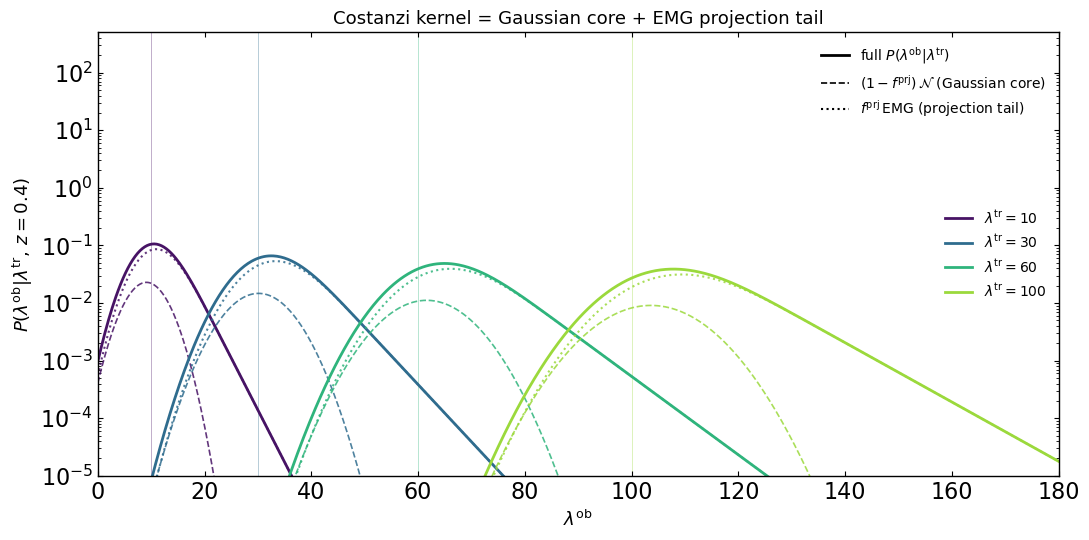
\includegraphics[width=0.85\linewidth]{../output/figs/02_projection_decomposition.png}
\caption{Decomposition of the kernel of Eq.~\ref{eq:c19-eq6} into its
$(1{-}f_{\rm prj})\mathcal N$ Gaussian core (dashed) and $f_{\rm prj}\,$EMG
projection tail (dotted) at $z = 0.4$ for four intrinsic richnesses
$\ltr \in \{10, 30, 60, 100\}$. The EMG tail rises with $\ltr$ and drives
the optical-selection bias on the lensing data vector.}
\label{fig:kernel-decomp}
\end{figure}

% ============================================================================
\section{Output 1 --- $N(\lob, \zob)$ number counts}
\label{sec:counts}

We obtain $N(\lob, \zob)$ by counting the mock halos that fall into each
$(\lob, \zob)$ bin on the DES~Y1 grid. Both axes are forward-model
outputs rather than catalog redMaPPer columns: the C19 sampler depends
only on $(M, z)$ and carries no per-halo LSS information, which matches
the inputs of the analytical $\Bcal_{\rm sel,C1}(\lob, \zob)$ of
\S\ref{sec:c1} and keeps the abundance and lensing sides of the data
vector in the same C26/C19 model world. $N(\lob, \zob)$ is therefore the
correct entry for a C26 likelihood integrating
Eq.~\ref{eq:lsat} into Eq.~\ref{eq:c19-eq6}.

% ============================================================================
\section{Lensing data vector --- ANALYTICAL route (Matteo / C26 Eq.~C1)}
\label{sec:c1}

\paragraph{Binning quantity.} The C19 forward-model $(\lob, \zob)$.
Each $\lob$ is an independent draw from the kernel of
Eq.~\ref{eq:c19-eq6} conditioned only on $(\ltr, z)$: the kernel
encodes the LSS-driven projection statistics through its EMG tail at
the population level, but per-halo $\lob$ values are not correlated
with the actual line-of-sight structure around each halo and therefore
carry no information correlated with the per-halo lensing signal.

\paragraph{Selection bias.} redMaPPer counts red-sequence galaxies inside
a projected aperture with no line-of-sight resolution, so projected LSS
preferentially boosts $\lrm$ for halos in over-dense filaments and lifts
the stacked $\Delta\Sigma(R)$ above the mass-only expectation. C26
Appendix~C captures this lift with a 5-parameter fitting function (no
integration); Matteo (priv.\ comm.) reports the same form fits the bias
on $\Delta\Sigma$:
\begin{equation}
\label{eq:c1-form}
  \Bcal_{\rm sel,C1}^{\Delta\Sigma}(R)
  = A\,\left(\frac{R}{R_0}\right)^{\!\alpha}
    \left[\,1 + \left(\frac{R}{R_0}\right)^{\!\gamma}\,\right]^{(\beta - \alpha)/\gamma}
    + C,
\end{equation}
with $(A, \alpha, \beta, \gamma, C) = (0.12,\, 4.11,\, -0.18,\, 1.82,\, 1.00)$,
$R_0 = R_\lambda(\lob)\,(1+\zob)$, and
$R_\lambda = (\lob/100)^{0.2}\,\hMpc$ (C26 Appendix~B).

The C26 paper writes the published form for $\Sigma$ with a fixed $+1$
rather than a free $C$ ($C = 1$ limit of Eq.~\ref{eq:c1-form}); we plot
both flavours for comparison. The data vector is
\begin{equation}
  \label{eq:c1-data-vector}
  \Delta\Sigma_{\rm obs}(R) = \Bcal_{\rm sel,C1}^{\Delta\Sigma}(R)\,
    \Delta\Sigma_{\rm stack}(R),\qquad
  \langle \gamma_t(R) \rangle = \Delta\Sigma_{\rm obs}(R)\,
    \Sigma_{\rm crit}^{-1}\!\left(\langle\zob\rangle_{\rm bin}\right),
\end{equation}
with $\Delta\Sigma_{\rm stack}$ the unweighted mean of \blk{DeltaSigma}
across the C19-binned halos in each $(\lob, \zob)$ cell.

\paragraph{Why a fitting function?} An MCMC chain evaluates the lensing
model $\sim 10^4$--$10^6$ times, so the per-step cost matters. Computing
the full Costanzi-2026 prediction from scratch requires nested integrals
over halo mass and redshift at every step --- prohibitive at chain
length. Equation~\eqref{eq:c1-form} replaces those integrals with five
constants per bin, cutting the cost from seconds to microseconds without
changing the answer.

\paragraph{Selection-bias ratio $\Bcal_{\rm sel,C1}^{\Delta\Sigma}(R)$}

The fitting function evaluated at the bin-mean $(\langle\lob\rangle,
\langle\zob\rangle)$ for every $(\lob, \zob)$ cell, with the published
$\Sigma$-flavour overlay.

\begin{figure}[H]
\centering
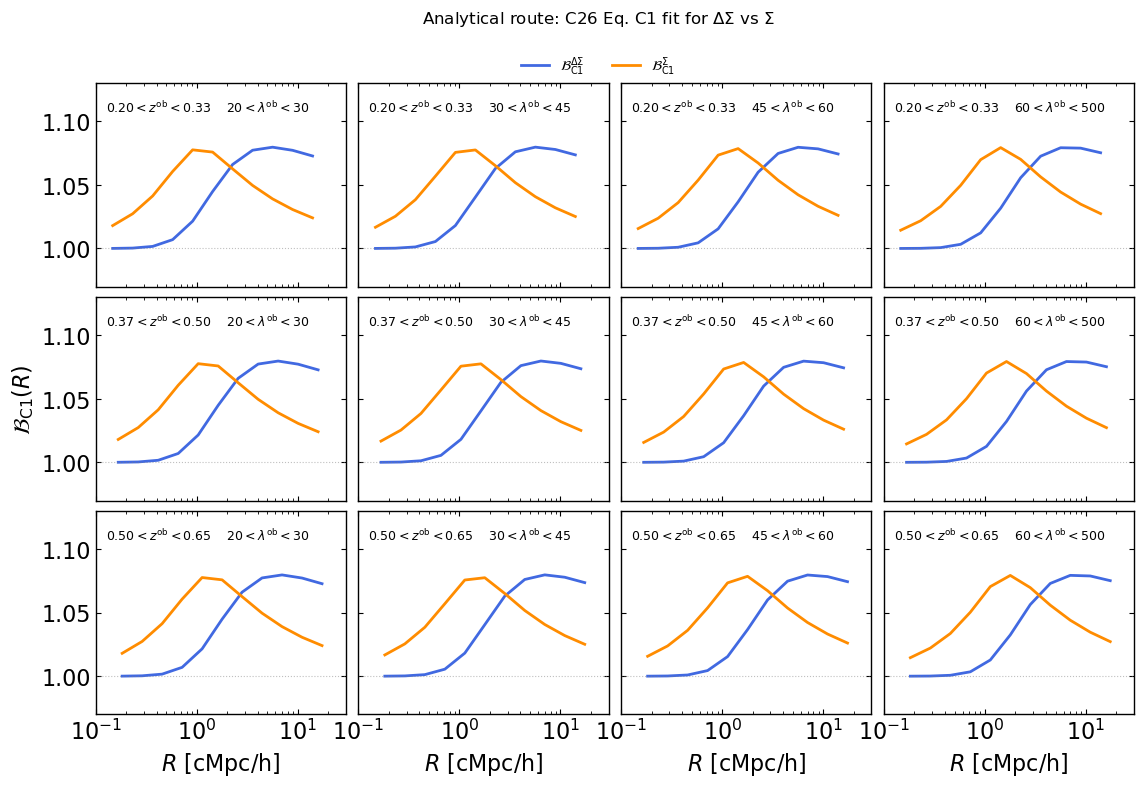
\includegraphics[width=0.95\linewidth]{../output/figs/03_analytical_Bsel_C1_ratio.png}
\caption{Analytical route: C26 Eq.~C1 selection-bias ratio per
$(\lob, \zob)$ bin on the DES~Y1 grid. Blue: $\Bcal_{\rm sel,C1}^{\Delta\Sigma}$
(used in the data vector). Orange: $\Bcal_{\rm sel,C1}^{\Sigma}$ overlay.
$x$-axis is comoving $R$ in $\hMpc$ to match the C26 convention; $y$-axis
is the bias factor.}
\label{fig:c1-ratio}
\end{figure}

\begin{comment}
\paragraph{Tangential shear with vs without the C1 correction}

\begin{figure}[H]
\centering
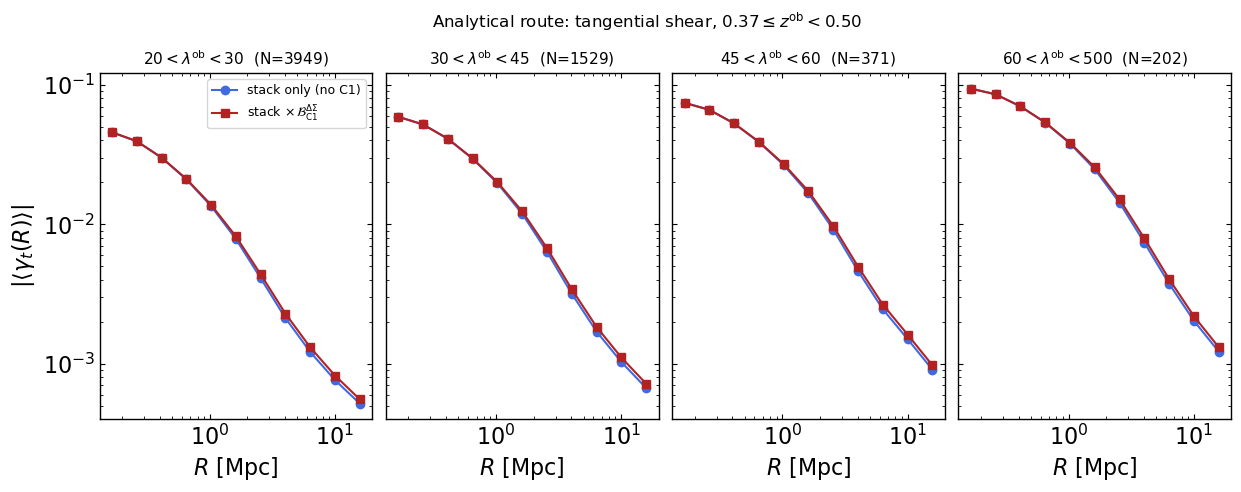
\includegraphics[width=0.95\linewidth]{../output/figs/04_analytical_shear_with_C1.png}
\caption{Analytical route: tangential shear in the middle redshift slice
$\zob \in [0.37, 0.50)$ for each richness bin. Blue circles: $\gamma_t$
from the unweighted C19-binned $\Delta\Sigma$ stack (no correction). Red
squares: same stack multiplied by $\Bcal_{\rm sel,C1}^{\Delta\Sigma}(R)$.
The C1 correction lifts the data vector by $\sim 5\text{--}15\%$
depending on bin and scale.}
\label{fig:c1-shear}
\end{figure}
\end{comment}

\subsection{Boost factor: member-galaxy contamination $B(R)$}
\label{sec:boost}

A real DES~Y1 measurement of $\Delta\Sigma$ is diluted by cluster-member
galaxies that survive photo-$z$ cuts and end up in the lensing source
catalog. These members carry no shear signal and reduce the measured
profile by the boost factor $B(R) \equiv 1/(1 - f_{\rm cl}) \ge 1$
(McClintock+2019 \S5.3.1). 
\begin{align}
B(R;\,r_s, b_0) &= 1 + b_0\,\frac{1 - f(x)}{x^2 - 1}, \qquad x = R/r_s, \nonumber \\[6pt]
f(x) &= \begin{cases}
\dfrac{\arctan\!\sqrt{x^2-1}}{\sqrt{x^2-1}}, & x > 1 \\[8pt]
\dfrac{\mathrm{arctanh}\!\sqrt{1-x^2}}{\sqrt{1-x^2}}, & x < 1
\end{cases}
\end{align}

To make the saved data vector mock the
\emph{raw uncorrected} DES~Y1 measurement, both lensing routes have
their final shear stack divided by $B(R)$:
\begin{equation}
  \langle\gamma_t\rangle^{\rm mock,obs} =
    \frac{\langle\gamma_t\rangle^{\rm obs}}{B_{\rm Y1\,data}(R)}
\end{equation}

\paragraph{Where $B_{\rm Y1\,data}(R)$ comes from.} The DES~Y1 cluster
analysis released measured boost-factor profiles per richness/redshift
bin, located at \pyfile{data/boost\_factor/profiles/}
(\texttt{full-unblind-v2-mcal-zmix\_y1clust\_l\{l\}\_z\{z\}\_zpdf\_boost.dat}).
The files are tabulated on an 11-point physical-Mpc $R$ grid
($0.166$ to $15.80$ Mpc); we adopt this grid as the global radial
axis for the saved data vector. The 7 cosmology-side richness bins
\texttt{l0..l6} include $\lambda < 20$ ranges; only \texttt{l3..l6}
match our 4 lensing bins
$\lambda \in \{[20, 30), [30, 45), [45, 60), [60, \infty)\}$. The
parametric McClintock+2019 Table~B1 fit is also computed (cell~42)
for sanity but is not used in the saved output.

\begin{figure}[H]
\centering
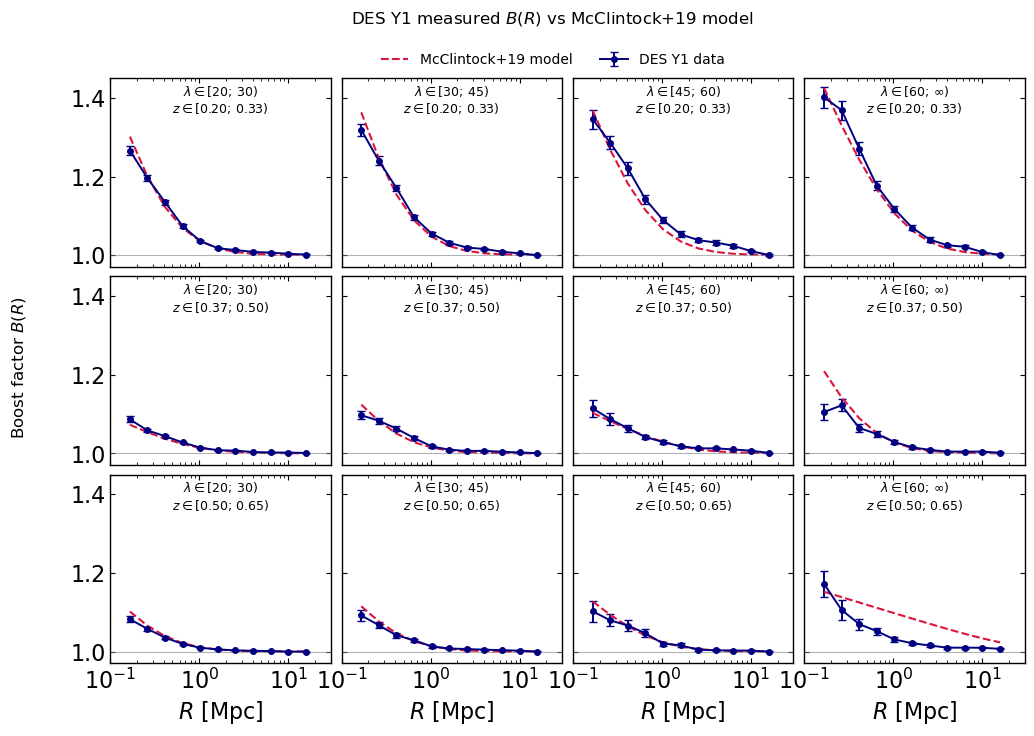
\includegraphics[width=0.95\linewidth]{../output/figs/08_boost_factor_data.png}
\caption{Measured DES~Y1 boost factor $B(R)$ per
$(\lambda^{\rm RM}, \zrm)$ bin with reported errors. Small-$R$ amplitude
rises with richness and falls with redshift, as expected for a
red-sequence-driven member contamination.}
\label{fig:boost-data}
\end{figure}

% ============================================================================
\section{Lensing data vector --- EMPIRICAL route (Heidi / mass-matched ratio)}
\label{sec:emp}

\paragraph{Binning quantity.} The catalog redMaPPer outputs
$(\lrm, \zrm)$, i.e.\ \blk{LAMBDA\_CHISQ} and \blk{Z\_LAMBDA}. These come
from running the redMaPPer cluster finder on the Buzzard photometric
catalog and \emph{do} carry per-halo LSS information.

\paragraph{Selection bias.} Built directly from the catalog as the ratio
of the redMaPPer-selected stack to a $(\log M, \ztr)$-matched random
reference, following Wu+2022 method iii
(\pyfile{src/stacked\_profile\_weighted\_by\_mass\_redshift.py}). For each
$(\lrm, \zrm)$ bin:
\begin{equation}
\label{eq:mass-match}
  \langle \Delta\Sigma(R) \rangle_{\rm rnd}
  = \frac{\sum_c w_c\, \langle\Delta\Sigma(R)|c\rangle_{\rm full\,mock}}
         {\sum_c w_c},\qquad
  w_c = N_c^{\rm sel},
\end{equation}
summed over $(\log_{10} M, \ztr)$ cells of width
$(\Delta\log M, \Delta z) = (0.1, 0.05)$. The cell averages are taken over
the \emph{full} mock, so the reference resamples halos that share the
selected sample's mass and redshift but were never preferentially picked
for their environment. The empirical bias is
\begin{equation*}
  \Bsel^{\rm emp}(R)
  = \frac{\langle \Delta\Sigma(R) \rangle_{\rm sel}}
         {\langle \Delta\Sigma(R) \rangle_{\rm rnd}}.
\end{equation*}
No fitting function, no $R \to 0$ extrapolation, both numerator and
denominator come straight from \blk{DeltaSigma}.

\paragraph{Bootstrap.} The reported $\Bsel^{\rm emp}(R)$ is the
\textbf{bootstrap mean} over $N_{\rm boot} = 50$ resamples of halos within
each bin (with mass-matched reference rebuilt at every step), capturing
the statistical uncertainty driven by finite halo count. The shaded bands
in the panel grids are the bootstrap standard deviation; the saved file
keeps only the bootstrap mean.

\subsection{Selection-bias ratio $\Bsel^{\rm emp}(R)$ with bootstrap bands}
\label{sec:emp-ratio}

We evaluate $\Bsel^{\rm emp}(R)$ on the redMaPPer-binned $(\lrm, \zrm)$
grid using Eq.~\eqref{eq:mass-match} and report the bootstrap mean and
$1\sigma$ band per bin. The expected signature is the bell-shaped excess
peaking near $R \sim 1$~pMpc that Wu+2022 (Fig.~2) identify as the
LSS-environment-driven selection bias: at smaller scales the one-halo
term dominates and the ratio approaches unity, while at larger scales
the projected over-density that boosted $\lrm$ falls outside the lensing
aperture and the ratio relaxes back toward one.

\begin{figure}[H]
\centering
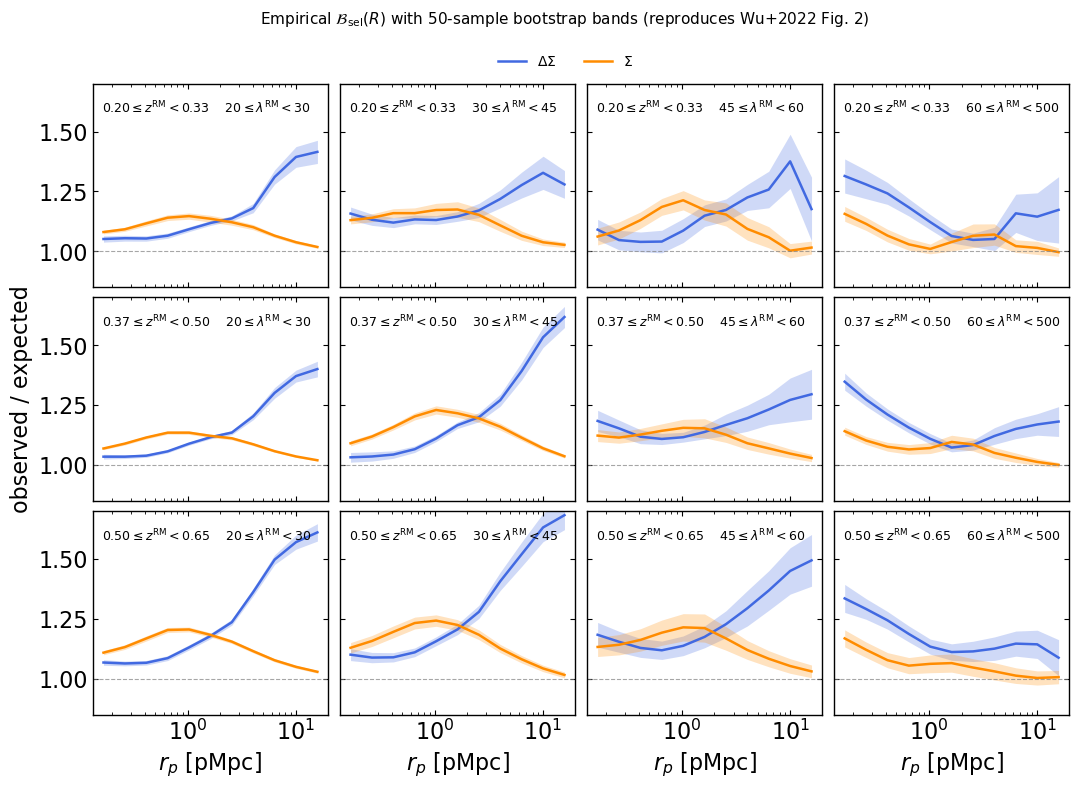
\includegraphics[width=0.95\linewidth]{../output/figs/05_empirical_Bsel_emp_bootstrap.png}
\caption{Empirical route: $\Bsel^{\rm emp}(R)$ per $(\lrm, \zrm)$ bin
on the DES~Y1 grid, with $N_{\rm boot}=50$ bootstrap bands. Blue:
$\Delta\Sigma$ ratio. Orange: $\Sigma$ ratio (overlay). Reproduces
Wu+2022 Fig.~2: the bell-shaped peak around $R \sim 1$~pMpc is the
LSS-environment-driven selection bias signal.}
\label{fig:emp-ratio}
\end{figure}

\subsection{Null test: replace $\lrm$ with the C19 sampler}
\label{sec:null}

If we re-bin on the C19 forward-model $(\lob, \zob)$ instead of the catalog
$(\lrm, \zrm)$, the same mass-matched-random pipeline should return
unity at every $R$, because the C19 sampler is by construction blind to
per-halo LSS. Any residual deviation from $1$ is the bias of the matching
procedure itself, not a physical signal.

\begin{figure}[H]
\centering
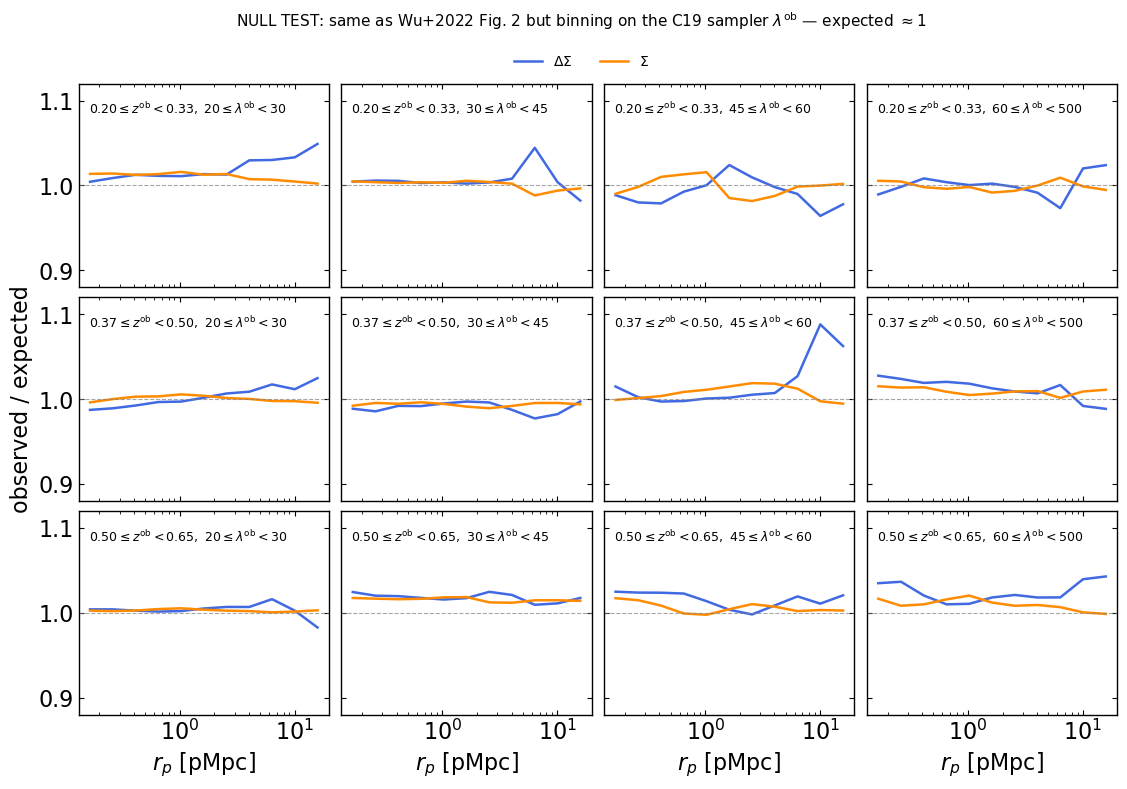
\includegraphics[width=0.95\linewidth]{../output/figs/06_empirical_null_test.png}
\caption{Null test: same Wu+22 panel grid but binning on the C19 sampler
$(\lob, \zob)$ rather than the catalog $(\lrm, \zrm)$. The bell collapses
to $\approx 1$ across all bins, confirming the $R \sim 1$~pMpc peak in
Fig.~\ref{fig:emp-ratio} is genuinely LSS-driven.}
\label{fig:null}
\end{figure}

\subsection{Tangential shear: redMaPPer-selected vs mass-matched random}
\label{sec:emp-shear}

The bias ratio of \S\ref{sec:emp-ratio} is most directly seen by
comparing the two tangential-shear stacks that enter its numerator and
denominator. The mass-matched random reference is the $\gamma_t$ a
hypothetical unbiased selector would measure on halos of the same
$(\log M, \ztr)$ distribution; the redMaPPer-selected stack is the
$\gamma_t$ an actual cluster finder produces. Their offset is the
observable counterpart of $\Bsel^{\rm emp}(R)$ and the quantity an MCMC
must reproduce.

\begin{figure}[H]
\centering
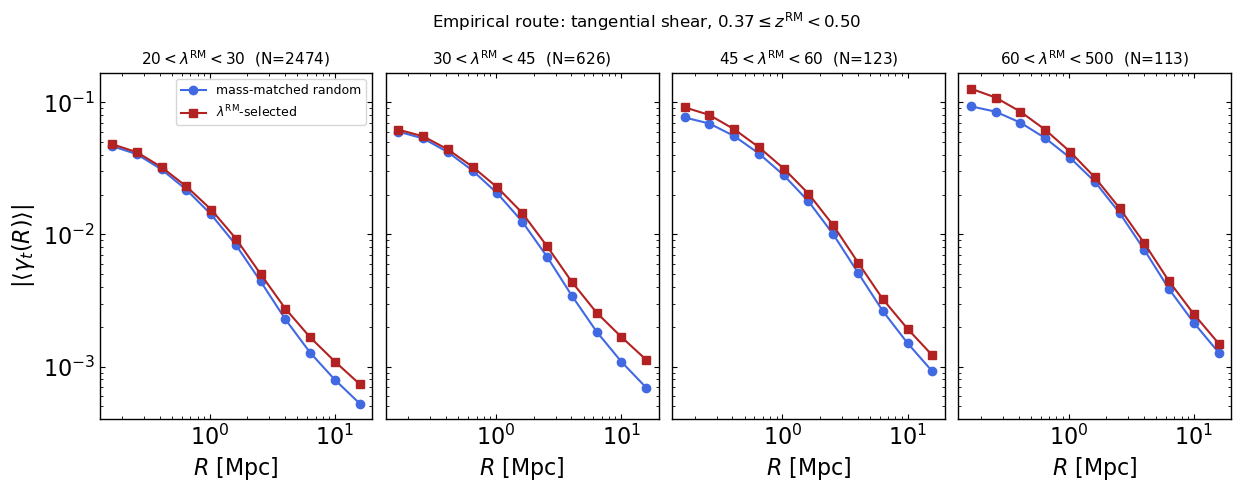
\includegraphics[width=0.95\linewidth]{../output/figs/07_empirical_shear.png}
\caption{Empirical route: per-bin tangential shear in the middle redshift
slice $\zrm \in [0.37, 0.50)$. Blue circles: $\gamma_t$ from the
mass-matched random reference. Red squares: $\gamma_t$ from the
$\lrm$-selected stack (the observed signal). The selected curve sits
above the reference by the $\Bsel^{\rm emp}(R)$ factor of
Fig.~\ref{fig:emp-ratio}.}
\label{fig:emp-shear}
\end{figure}

% ============================================================================
\section{Output archive}
\label{sec:archive}

The final notebook cell writes both routes plus bin metadata to a single
\pyfile{output/MockDataVector.npz}. With $N_\lambda = 4$, $N_z = 3$,
$N_R = 11$ (DES~Y1 boost-factor profile grid):

\begin{table}[H]
\centering
\small
\begin{tabular}{@{}l l p{0.45\linewidth}@{}}
\toprule
Key & Shape & Content \\
\midrule
\multicolumn{3}{l}{\textit{Bin metadata}}                                                       \\
\blk{radii\_phys\_mpc}    & $(N_R,)$               & 11-pt DES~Y1 boost grid (physical Mpc; $0.166$--$15.80$) \\
\blk{lambda\_bins}        & $(N_\lambda + 1,)$     & DES~Y1 richness edges $\{20, 30, 45, 60, 500\}$ \\
\blk{z\_bin\_min}         & $(N_z,)$               & lower-redshift edges \\
\blk{z\_bin\_max}         & $(N_z,)$               & upper-redshift edges \\
\midrule
\multicolumn{3}{l}{\textit{Number counts (DES~Y1 expectation)}}                                 \\
\blk{NC}                  & $(N_\lambda, N_z)$     & $N(\lob, \zob)$, Buzzard counts rescaled by $\Omega_{\rm Y1}(z)$ \\
\midrule
\multicolumn{3}{l}{\textit{Analytical route, C19-binned}}                                       \\
\blk{gamma\_t\_stack\_C19} & $(N_\lambda, N_z, N_R)$ & stacked $\gamma_t$, no correction \\
\blk{gamma\_t\_obs\_C1}    & $(N_\lambda, N_z, N_R)$ & stack $\times\, \Bcal_{\rm sel,C1}^{\Delta\Sigma}$ \\
\blk{B\_sel\_C1}           & $(N_\lambda, N_z, N_R)$ & analytical $\Bcal_{\rm sel,C1}^{\Delta\Sigma}(R)$ \\
\midrule
\multicolumn{3}{l}{\textit{Empirical route, RM-binned}}                                         \\
\blk{gamma\_t\_stack\_RM}  & $(N_\lambda, N_z, N_R)$ & $(\log M, \ztr)$-matched random reference $\gamma_t$ \\
\blk{gamma\_t\_obs\_RM}    & $(N_\lambda, N_z, N_R)$ & $\lrm$-selected stack $\gamma_t$ (the observed signal) \\
\blk{B\_sel\_emp}          & $(N_\lambda, N_z, N_R)$ & bootstrap-mean $\Bsel^{\rm emp}(R)$ \\
\midrule
\multicolumn{3}{l}{\textit{DES~Y1 boost factor + final mock-observed shears} (\S\ref{sec:boost})} \\
\blk{B\_data}                & $(N_\lambda, N_z, N_R)$ & measured DES~Y1 $B(R)$ \\
\blk{B\_data\_err}           & $(N_\lambda, N_z, N_R)$ & 1-$\sigma$ error per radial bin \\
\blk{B\_data\_cov}           & $(N_\lambda, N_z, N_R, N_R)$ & full radial covariance matrix per bin \\
\blk{gamma\_t\_mock\_obs\_C1} & $(N_\lambda, N_z, N_R)$ & analytical (Matteo) shear with Y1 boost dilution \\
\blk{gamma\_t\_mock\_obs\_RM} & $(N_\lambda, N_z, N_R)$ & empirical (Heidi) shear with Y1 boost dilution \\
\bottomrule
\end{tabular}
\caption{Output-archive layout. Default shapes are $(4, 3)$ for the
counts and $(4, 3, 15)$ for the radial vectors.}
\label{tab:archive}
\end{table}

% ============================================================================
\section{Known simplifications}
\label{sec:future}

\begin{itemize}
  \setlength\itemsep{2pt}
  \item \textbf{Photo-$z$ kernel.} The Gaussian
    $\sigma_z = 0.01\,(1+\ztr)$ proxy is a stand-in for the
    redshift- and colour-dependent kernel of Myles+2021. It captures
    the dominant scatter but misses the tails that drive the
    high-$z$ outlier rate.
  \item \textbf{Boost factor uses DES~Y1, not Y3, measurements.}
    \S\ref{sec:boost} injects $B(R)$ from McClintock+2019 Y1 profiles,
    which is the closest released measurement matching our cluster
    binning. A Y3 boost-factor measurement is not yet released; when
    it is, swap the source files in \pyfile{data/boost\_factor/profiles/}
    without further code change.
  \item \textbf{Posterior-mean projection coefficients.} The C19
    projection parameters are evaluated at the posterior mean of the
    upstream chain. Row-by-row covariance propagation is not
    implemented.
  \item \textbf{Single Y3 realisation.} The §8.1 empirical ratio is
    computed on one Y3 realisation; Wu+2022 averages 12 Y1 + 1 Y3
    realisations and is correspondingly tighter.
\end{itemize}

% ============================================================================
\section{File map}
\label{sec:files}

\begin{itemize}
  \setlength\itemsep{1pt}
  \item \pyfile{MockDataVector.ipynb} --- the production notebook.
    Top-to-bottom execution reproduces every figure and writes the
    output archive.
  \item \pyfile{src/costanzi\_selection.py} --- C26 Eq.~15 sampler and
    C19 Eq.~6 mixture sampler, plus the legacy single-scale $\Bsel$
    weight.
  \item \pyfile{src/stacked\_profile\_weighted\_by\_mass\_redshift.py} ---
    Wu+22 / Esteves $(M, z)$-matched random reference builder.
  \item \pyfile{src/radial\_bins\_phys\_mpc.py} --- the 15-bin physical
    radial grid \blk{rp\_phys\_mpc}.
  \item \pyfile{data/prj\_params\_DESY3\_lss\_lin\_dep\_getdist\_v1.txt}
    --- 15 posterior samples of the 10 C19 projection coefficients.
  \item \pyfile{src/fileLoc.py} --- machine-resolved path table for the
    raw Buzzard halo catalogue, profile output, and $\beta_{\rm eff}$
    table.
  \item \pyfile{output/MockDataVector.npz} --- saved data vector
    (Tab.~\ref{tab:archive}).
  \item \pyfile{output/figs/} --- headline plots embedded in this PDF.
  \item \pyfile{docs/MockDataVector.tex} --- this document.
\end{itemize}

\section{References}
\label{sec:refs}

\begin{itemize}
  \setlength\itemsep{1pt}
  \item Costanzi et al.\ 2026, \emph{Forward analytical model for the
    optical selection bias on galaxy cluster lensing profiles}.
    Eqs.~15 (mass--richness), Appendix~C Eq.~C1 (selection-bias fit),
    Sec.~III (Poisson--Gaussian convolution).
  \item Costanzi et al.\ 2019, arXiv:1807.07072. Eq.~6 (Gaussian + EMG
    mixture), Appendix~A Eq.~A8 (per-parameter forms).
  \item Wu et al.\ 2022, arXiv:2203.05416. Fig.~2 (selection-bias panel
    grid) and Appendix~B (mass--redshift weighted reference).
  \item McClintock et al.\ 2019, MNRAS 482, 1352 --- DES~Y1 cluster
    binning convention used throughout.
\end{itemize}

\end{document}
